% 2013 年北京卷理科第 11 题：圆的切线与割线。
% 来源 PDF：普通高考/2013/2013北京理.pdf，第 1 页（印面 787）中栏。
% AB 为圆 O 的直径，PA 切圆于 A，PB 与圆交于 D；PA=3，PD:DB=9:16。
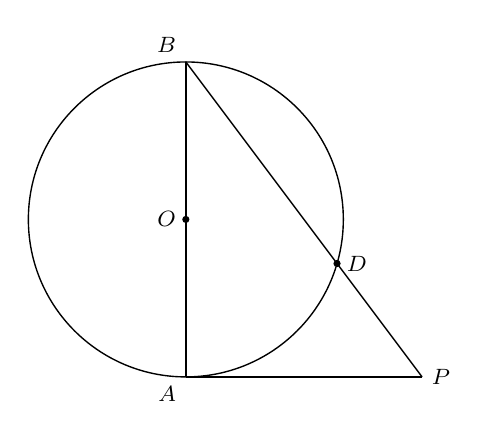
\begin{tikzpicture}[font=\footnotesize, line width=0.5pt, scale=1]
  \coordinate (O) at (0,0);
  \coordinate (A) at (0,-2);
  \coordinate (B) at (0,2);
  \coordinate (P) at (3,-2);
  \coordinate (D) at (1.92,-0.56);
  % 圆
  \draw (O) circle (2);
  % 直径 AB
  \draw (A) -- (B);
  % 切线 PA 与割线 PB
  \draw (P) -- (A);
  \draw (P) -- (B);
  % 点
  \fill (O) circle (1.3pt);
  \fill (D) circle (1.3pt);
  \node[left] at (O) {$O$};
  \node[below left] at (A) {$A$};
  \node[above left] at (B) {$B$};
  \node[right] at (P) {$P$};
  \node[right] at (D) {$D$};
\end{tikzpicture}
